\chapter{Proposed approach}
\label{CapFT}

\section{Theoretical part}

\subsection{Architecture}

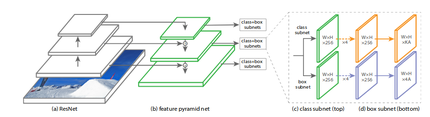
\includegraphics{Fig/arch1.png}

The model our work is based on is RetinaNet.
RetinaNet is a one stage detector having a convolutional neural network as a feature extractor for the 2 task-subnetworks it has. 
The first CNN's backbone is based on a Feature Pyramid Network build on a forward Residual Network. The FPN generates rich multi-scale feature 
maps. In [7] it is emphasised that we can also extract relevant features and make predictions based on feature maps that are on layers 
inside the network.
The pyramid usually has 7 levels.
The 2 task-subnetowrks are:
\begin{itemize}
  \item The classification subnetwork is a FCN that appears on each level of the pyramid and tries to classify each anchor box and outputing a K-vetor of probabilities for each class(meaning we have K classes).
  \item The box regression subnetwork has the same architecture (but different parameters) like the classification subnetwork only outputing a 4-vector representing the targets of the bounding box.
\end{itemize}

\subsection{The loss}

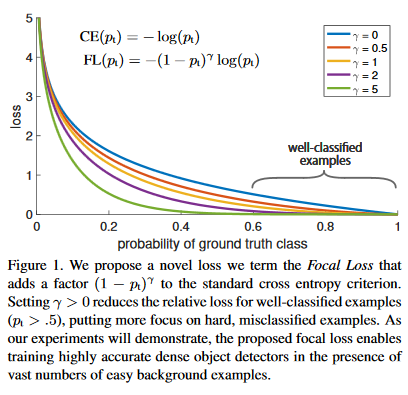
\includegraphics{Fig/focalloss.PNG}

Instead of the cross-entropy loss function we used a more novel loss function called the focal loss. The reason behind using focal loss is that (instead of using Online Hard Example Mining) the loss emphasies learning from hard examples.
The focal loss function stands at the end of the classification FCN and applied to all 100k anchor boxes sampled from a single image.

\section{Application development}

